\nnarticleheader{Foundations of Mathematics: Part II}{Dr. Mark Gottlieb, Haverford Faculty}
% hello from the past! remember to include this article in Issue V of the notebook. maybe add a little blurb before the next section about how this is a continuation of last year's article. best of luck! ~past Greer

\begin{center}
	\textit{The following article is Part II of Dr. Gottlieb's "Foundations of Mathematics"\\ 
	(inclding sections on \textbf{Formalism} and \textbf{Constructivism}).\\
	To read Part I (\textbf{Formalism} and \textbf{Constructivism})\\
	check out Issue IV of Newton's Notebook.}
\end{center}


\noindent
\textbf{Formalism}

    If mathematicians aren't studying unchanging objects or working out logical deductions, what are they doing?  We seem to be running out of possible ways of understanding what mathematics is all about.  In fact, there are other possibilities.  Some mathematicians, beginning about eighty years ago and inspired by the German mathematician David Hilbert, have argued that mathematics is really just a very complex game--the manipulation of symbols on paper according to rules.  The Transitive Property of Equality, mentioned above, is one example of this kind of rule, called a rule of inference.  Mathematicians who believe that mathematics is just a game with symbols are called \emph{formalists}.  Whereas Platonism and logicism never convinced the majority of mathematicians, for most of the twentieth century most mathematicians considered themselves formalists.  Both in the research papers they wrote and in the textbooks they authored, their approach was formalistic.  They communicated this way of thinking about mathematics to their students, and until recent decades, it dominated the advanced study of mathematics and mathematics education at other levels, as well.
     
     There are a number of peculiar consequences of the formalist view of mathematics.  One of the strangest is that formalists do not believe that mathematics is about numbers, spatial relationships, and patterns.  Instead, they will tell you that mathematics is really about 'marks on paper'.  Notice that they do not assign any meaning whatsoever to these marks--they might as well be gibberish.  As long as I follow the rules of inference correctly, according to formalists, I am a good mathematician.  When they are asked what numbers, triangles, and functions are, formalists reply, "Just names for symbols on a piece of paper."   Mathematical research, on the formalist view, is figuring out what new sets of symbols can be produced from the sets we already have using given rules of inference.\footnote{Interestingly, this seems to imply that computers could be quite good mathematical researchers, as they are essentially symbol-manipulating machines that follow formal rules.  A program that could check every mathematical statement for truth or falsity could do away completely with the need for human researchers in pure mathematics.}
     
      This explanation seems to conflict with the common experience we have when we are doing mathematics that we are thinking about numbers, shapes, and patterns, not just symbols.  For example, when we try to understand the properties of a number (like whether or not it is prime) or a shape, we often use our imagination to "turn things over in our mind".\footnote{The Dutch mathematician L.E.J. Brouwer was so impressed by this ability that he created an entire philosophy of mathematics called intuitionism.  Brouwer believed that all mathematical knowledge was based upon a direct intuition of the natural numbers.  Earlier versions of this theory can be found in the works of the great German philosopher, Immanuel Kant, and the mathematician Richard Dedekind.  Today few mathematicians accept Brouwer's approach, as it introduces a number of logical peculiarities.  For a brief survey, see Howard Eves, \textit{Foundations and Fundamental Principles of Mathematics}, pp.}  We think about breaking up the number in diferent ways, or we imagine the triangle in different positions.  From this mental process, we may discover new facts about numbers or triangles.  Mathematicians speak of "mathematical intuition" that enables them to make new discoveries or new conjectures.  This kind of intuition is a bit like having a hunch, a good understanding of a situation without spelling out all the details.  Sometimes we can just "see" that something is true without being able to say why.   Formalism essentially does away with the idea of mathematical intuition.  If mathematics is just moving symbols around, there doesn't seem to be any place for intuition about mathematical objects.  In fact, there isn't even a place for mathematical objects to begin with.
        
     When it comes right down to it, according to formalists, mathematics is really just making calculations.  Some of these calculations, or computations, as they are called in computer science, are simple, like multiplying 213 x 123.  Computations can, however, become very complicated, like figuring out whether or not a particular set of symbols follows by rules of inference from a set of basic symbols.
       
A program is a set of instructions that tells a computer to perform a list of operations in a specific order.  All programs have the same basic purpose: to turn input into output.  The computer receives input, it executes or carries out the program, then it displays an output.  For example, if my program tells the computer to multiply a number by 12, and my input is "7", the computer will display the output "84".  Mathematicians have developed a concept to express this relation of input to output, the well-known concept of a function. It is one of the most important of all mathematical ideas.  Here is the definition.
\begin{dfn}
A \emph{function} is a set of ordered pairs $(x,y)$ such that to each value of $x$ there corresponds one and only one value of $y$.  We often think of the value $x$ as being the input to the function, and $y$ as being the output.  (Note that $x$ and $y$ may or may not be numbers.)
\end{dfn}

We say, "$y$ is a function of $x$" if and only if the set of ordered pairs $(x,y)$ is a function and use the notation $ y=f(x) $ to indicate that $y$ is a function of $x$.  This means that $x$ is the input to the function and $y$ is the output.  We call the function $f$ and we can think of $f$ as being a rule that tells us how to compute the output $y$ from the input $x$. The set of all input values to a function is called the \emph{domain} of the function.  The set of all output values is called the \emph{range} of the function.

\begin{exm}{3}
The set $\{(1,2), (5,7), (7,\pi)\}$ is a function.  To each input there corresponds one only one output.  The domain is the set \{1,5,7\}, and the range is the set $\{2,7,\pi\}$.  If the first number in the ordered pairs is called $x$ and the second $y$, then we can write $y = f(x)$.
\end{exm}
\begin{exm}{4}
A function can be defined by an explicit rule.  Here is a simple case: $T(C) = 1.8C + 32$.  In this case we think of $C$ as being the input to the function and $T$ as being the output.  Some ordered pairs are ($0, 32)$, ($5, 41)$, and ($100, 212)$.  This function comes from the physical sciences.  Do you recognize it?
\end{exm}
\begin{exm}{5}
By plotting the ordered pairs deriving from a function we can generate the graph of a function.  In the above case we have:
\begin{center}
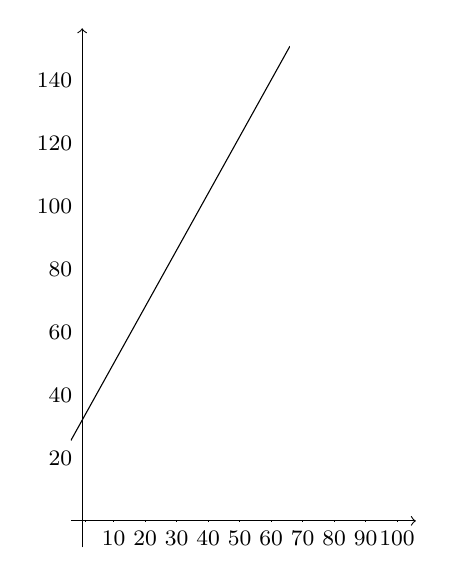
\begin{tikzpicture}[scale = 0.04][line cap=round,line join=round,>=triangle 45,x=1.0cm,y=1.0cm]
\draw[->,color=black] (-3.6,0) -- (105.97,0);
\foreach \x in {,10,20,30,40,50,60,70,80,90,100}
\draw[shift={(\x,0)},color=black] (0pt,2pt) -- (0pt,-2pt) node[below] {\footnotesize $\x$};
\draw[->,color=black] (0,-8.4) -- (0,156.45);
\foreach \y in {20,40,60,80,100,120,140}
\draw[shift={(0,\y)},color=black] (2pt,0pt) -- (-2pt,0pt) node[left] {\footnotesize $\y$};
\clip(-3.6,-8.4) rectangle (65.97,156.45);
\draw [domain=-3.6:65.97] plot(\x,{(--32--1.8*\x)/1});
\end{tikzpicture}
\end{center}
\end{exm}
\begin{exm}{6}
A function can be defined by a table of values, like the following:
\begin{center}
\begin{tabular}{|c|c|}
\hline 
$x$ & $y$ \\ 
\hline 
1 & 1 \\ 
\hline 
5 & 4 \\ 
\hline 
9 & 5 \\ 
\hline 
13 & 17 \\ 
\hline 
\end{tabular} 
\end{center}
Here, we can see that $y$ is a function of $x$, since to each $x$ corresponds one and only one $y$.  The domain is $\{1,5,9,13\}$ and the range is $\{1,4,5,17\}$.  A challenging problem is to come up with an explicit rule for the function.
\end{exm}
Armed with the idea of a function, we can better understand the formalist idea of mathematics and some of its limitations.  If mathematics is just rule-governed operations with symbols, then it looks as though it could be done by a computer without any help from a human being.  In fact, that's exactly what computers do; they perform operations on strings of symbols according to rules.  We input a string of symbols, press "Enter" and out comes another string of symbols.  In short, if formalists are right, mathematics could be done completely by machines, and human mathematicians would be unnecessary.

How would these machines work?  We would write a complicated program to figure out whether a particular string of symbols was a theorem.  Remember, a theorem is the conclusion of a formal proof, the last statement in a chain of logical steps. Our program, called a \emph{theorem-proving program}, would be able to check any string of symbols to determine whether or not it was a theorem. We could call this function T.  Its domain would be the set of all strings of symbols allowed in our symbol system, and its range would be 
\begin{center}
$\{\text{theorem},\text{not theorem}\}$
\end{center}   

For example, if the string of symbols  
\begin{center}
$\sigma\mu\kappa\upsilon\varsigma\Gamma$
\end{center} 
were a theorem in our system, we when we ran our program we would get
\begin{center}
$T(\sigma\mu\kappa\upsilon\varsigma\Gamma)= \text{theorem}$
\end{center} 
Once again, this means that the string '$\sigma\mu\kappa\upsilon\varsigma\Gamma$' can be derived from our basic assumptions by following the rules of inference.

The goal of the formalists was to show that all of mathematics can be represented by system of symbols and rules of inference.  All that was needed, they believed, was to find the right set of symbols and inference rules.  It is a remarkable fact that this goal turns out to be impossible.  In 1931 Kurt G\"{o}del (1906-1978), an Austrian logician, proved, using traditional mathematical methods, that, regardless of how we set up our system, there will always be certain strings of symbols that are neither theorems nor non-theorems in our system, but may recognized as true or false by mathematicians. 

In other words, our function $T$ simply won't work for those strings.  Mathematicians call G\"{o}del's result an \emph{Incompleteness Theorem}, because it shows that there is no way to create a formal system that can determine for any string of symbols it contains whether or not that string is a theorem.  There will always be strings of symbols that are `undecidable' in every formal system.  
G\"{o}del's work showed that mathematics cannot be completely turned over to machines, like computers, because there will always be some strings of symbols whose correctness can only be assessed by human beings.  There is no way to build a machine which we can be sure will be able to prove all true mathematical statements starting from a single set of assumptions.  To G\"{o}del, this result meant that mathematics must be something over and above any kind of symbolism.  This led him to become a Platonist, as we mentioned earlier.  G\"{o}del's basic idea was to show that all theorem-proving programs run into insurmountable problems when faced with statements like, "This statement is false."  This is similar to the difficulty we encountered in our discussion of Russell's Paradox.

\noindent
\textbf{Constructivism}

It looks as though none of the approaches we have so far considered gives an entirely adequate account of the nature of mathematics.  To summarize, we have seen that mathematics cannot be about things that are completely separate from the physical world; it is not purely logical, and it seems to be more than just a collection of symbols.  During the latter half of the twentieth century it became increasingly clear that none of the traditional ideas about mathematics were entirely correct.  Some mathematicians began to suggest that, perhaps, mathematics is a much more complex activity than anyone had imagined.  In fact, it began to look like each of the traditional ideas covered only part of mathematics. 
 
     A number of mathematicians and philosophers in recent years have suggested that to understand mathematics we will need to take its many different aspects into account.  Above all, these mathematicians suggest that mathematics is a human creation. Let us call this point of view \emph{social constructivism}.  Its chief proponents include the Hungarian mathematician Imre Lakatos, the British philosopher Karl Popper, and Paul Ernest, a British educational theorist.  According to these men, our mathematical knowledge does not rest on unshakeable foundations, like a direct awareness of numbers or shapes, as the Platonist and intuitionist  claim.  Neither does it rest upon logic or basic facts about sets.  Instead, constructivists believe that mathematics is a creative product of human activity.  They believe that numbers, geometrical shapes, and mathematical patterns were invented by human beings, originally for the purpose of solving practical problems.  For example, the Egyptians introduced the right triangle to assist them in agriculture and architecture; the Babylonians introduced numerals as aids to counting and record-keeping. 
      
     At first triangles and numerals were only tools, like hammers and saws.  Eventually, however, people began to raise questions about the relationships between the parts of a triangle or about whether or not a particular number was prime.  These questions have correct answers, and those answers do not depend upon anyone's opinion.  Human beings invented numbers, according to constructivists, but they did not invent the \emph{properties}, or basic facts about, numbers.  Once numbers have been invented, they come to have a life of their own, much like words, or laws, or Shakespeare's plays.  Constructivists speak of mathematical problems as "autonomous", meaning that they are not invented by us.  Once mathematical ideas have been invented, certain kinds of questions naturally arise.  These questions lead to investigation, to making educated guesses or conjectures, and to efforts to develop proofs.  Lakatos writes, 
\begin{quote}
          mathematics does not grow through a monotonous increase of the
          number of indubitably established theorems, but through the incessant
          improvement of guesses by speculation and criticism, by the logic of 
          proofs and refutations. \footnote{Qtd. in Hersh, \textit{What is Mathematics, Really?}, p. 211 }
\end{quote}  
          
Mathematical results are consequences of our invention of mathematics, but they are unintended consequences.  In other words, mathematics grows and changes in unpredictable ways as we work at it.  This, of course, is also true of other human activities; as Popper says, we often get more out than we put in. 
 
For example, as an artist works on a painting, the development of the painting affects how he does his work.  He might not realize that he was really painting a self-portrait when he thought she was painting a portrait of someone else.  She  doesn't realize this until she begins actually to put paint on the canvas and sees how things are turning out.  As another, more mathematical, example consider a complex game, like chess.  All the rules of chess are man-made, products of the human mind.  Nevertheless, as you may be aware, there are many principles or main ideas of chess strategy that were not completely understood until the game had been played for thousands of years.  These principles were not deliberately included in the rules; they were unintended consequences.  Einstein once remarked, "My pencil is cleverer than I am."  He meant by this that he often did not see the consequences of his ideas until he put them down on paper and began to work with them.  According to constructivists, the same is true of mathematics:  we do not fully understand mathematical ideas until we begin to work with them.  Thus, on a constructivist view, a proper mathematical education will not have its basis in mastering an established body of mathematical knowledge by rote but, rather, will emphasize the importance of the student's reconstructing the process of mathematical discovery underlying fundamental results.  In working results out for himself, the student is able to participate directly in the act of effectively employing mathematical tools and, perhaps--in extraordinary cases--advancing the development of mathematics itself, if only by criticizing standard assumptions.

The great strength of constructivism lies clearly in the emphasis it places upon the informal, creative, and evolving nature of mathematical thought, aspects that are all but neglected by the approaches considered earlier.  To be sure, constructivists have been quite right to emphasize the informal, creative, and evolutionary nature of mathematical thought.  It is undoubtedly true that classical approaches to mathematical thinking have almost universally been guilty of treating mathematical ideas as though they arrived ready-made in the human mind, whereas it has only been by a lengthy process of trial and error, of conjecture and refutation, that mathematics has reached its present form.  But there is a great difference between describing the process of mathematical discovery and describing the body of knowledge discovered.  If mathematical knowledge is, as constructivists maintain, a product of human convention, it is clearly a most extraordinary product.  It is true that certain social conventions, like language, customs of dress, or even traffic laws may come, in time, to seem to be both universal and necessary, but as American drivers may recognize when traveling in Britain, or French speakers in Germany, these conventions are quite easily given up when the circumstances require it.  

This is not true, however, of mathematical judgements, which seem to hold in all places and times and to admit of no possible alternatives.  It seems to be both certain and necessary that, for example, $7 + 5 = 12$.  There seems to be no question of giving up
our belief in this statement.  It is simply inconceivable, short of confusion, that we should believe that $7 + 5 = 13$.  This inconceivability accounts, in large part, for
the apparent necessity of mathematical truths.
  
Constructivists, as we have seen, are well aware of the special status of mathematical knowledge, and, as indicated above, have generally explained the apparent objectivity and universality of mathematics by holding that the relationships among mathematical ideas are not man-made, although the ideas themselves are.  But this view really is not very different from that of the logicists, namely, the view that mathematics consists of nothing more than drawing logical conclusions from given assumptions.  The assumptions may be man-made ideas, but the process of discovering relations between them is not distinguishable from logic, and we saw earlier that logic does not completely capture the nature of mathematical activity.  Constructivism contains important insights, but it fails as a complete framework for understanding the nature of mathematics. 

\noindent
\textbf{Conclusion: One Discipline, Many Faces}

 During the latter years of his life, the philosopher Ludwig Wittgenstein, one of the most influential thinkers of the twentieth century, became well known for his opposition to the notion that it is, or ought to be, possible to state precise definitions of terms employed in our ordinary experience.  Thus, speaking of the term "game", for example, we might attempt the following definition: "a competive activity aiming at a goal".  But solitaire is a game, and it is not competitive.  Moreover, frisbee is a game, but its "goal" is far from obvious.  In this way, our efforts at definition may come to nought.  Nevertheless, games do indeed share what Wittgenstein called a 'family resemblance' by which we are able to recognize them.  This resemblance may not be easily articulated, and there may well be cases which seem to lie at the periphery (Is surfing a game?), but most competent users of our language would agree about what constitutes a game and what does not (Performing brain surgery is \textbf{not} a game.)  There are good reasons for supposing that mathematics has much the same nature.
 
     We have seen that the most strenuous efforts of mathematicians to define their subject in straightforward terms have not been successful, or, more, correctly, have only been partially successful.  In the last analysis it seems fair to say that each of the principal approaches to the foundations of mathematics has identified one aspect of mathematical thought and constructed an account that places a more or less exclusive emphasis on that aspect.  For example, Platonism derives its plausibility from emphasizing the apparent objectivity, universality, and necessity of mathematical knowledge.  On the other hand, logicism is rooted in the observation that mathematics is the most logically rigorous branch of human knowledge, exhibiting the highest possible degree of structure, coherence, and rationality.  It is this deductive structure that makes mathematics universally applicable to other fields and enables mathematical thinking to be employed in all walks of life.  Mathematics is unique among disciplines in its use of precisely defined terms and symbols.  In no other field of human activity is symbolism employed in such a manner. This, no doubt, accounts for the appeal of formalism to a generation of eminent mathematicians.  Finally, mathematics has much in common with both art and science.  With the arts, mathematics shares a deep sense of aesthetic value; nearly all mathematicians would agree that their subject is beautiful.  Furthermore, like the arts, mathematics is a creative discipline, with new ideas and methods constantly being developed.  Like the sciences, mathematics is in pursuit of truth, and any mathematical conjecture is subject to criticism and revision, much like  a scientific theory.  Like great theoretical ideas in the sciences, mathematical ideas that unify seemingly disparate branches of the discipline represent the supreme intellectual achievement of the mathematician.
     
It seems then, that mathematics has not yet been defined adequately.  Perhaps the search for such a definition is fundamentally misguided, or perhaps an ingenious mind may someday adequately express the nature of mathematics.  Whatever may be the case,  several aspects of mathematics will be  especially important to its growth and development in the 21st century.  Let us discuss each of these in turn.
     
First, although its applications will increase exponentially in the future, mathematics will continue to be an inherently abstract discipline, and its level of abstraction will continue to rise.  The abstract nature of mathematics, though often an obstacle to the layperson, is precisely what gives mathematics its universal power to act as a model for nearly every aspect of reality, from the large-scale structure of space-time to the complex workings of nervous systems to the behavior of the nuclei of atoms.   It is nothing short of amazing that on many occasions discoveries of mathematicians working at problems belonging to "pure" mathematics have become cornerstones of scientific theories and technological advances of the widest significance.  This process began in the seventeenth century with Newton's and Leibniz's work on integral calculus and reached a pinnacle in the application of the abstract geometry of Riemann to Einstein's General Theory of Relativity.  Spectacular examples in recent times include the development of the modern computer from the theoretical ideas of Alan Turing, a British mathematician, as well as the ingenious use of binary numbers to make possible the Information Age.
      
Second,  mathematics will continue to grow, generating new methods, concepts and problems.  Its growth will be twofold.  On the one hand, it will be driven by imperatives deriving exclusively from mathematics itself and the many unsolved problems that continue to attract the best mathematical minds.  While solutions are are clearly desirable, as a by-product of ongoing reseach new questions are almost certain to arise and generate yet more unsolved problems.  In this way, the field of mathematical inquiry enlarges and deepens in scope.
       
Mathematical work will also be stimulated by the drive to master the complexities of both the natural and the human world.  This imperative will come not only, as it has traditionally, from physics, but also, and increasingly, from molecular biology, medicine, economics, and neuroscience.  The advent of ever-greater computing power will make it possible to model in real time (or hyper-real time) such phenomena as information processing in the visual cortex, the pharmacological effects on the body of new medicines, and the behavior of large-scale social and economic systems.  At the outer limit we can imagine mathematical models so powerful they can emulate the human mind, both in its cognitive and affective aspects.  We are pursuing that goal today, and the prospects are good that we will attain it, provided we have the insight and ingenuity.

     In the coming century mathematical thought will be, more than ever before, intimately linked to its embodiment in technology.  To be sure, mathematics has always been a calculational science. Geometry takes its name from surveying the earth, while trigonometry has similar origins; in modern times we have the logarithms of Napier, the calculus of Newton, and Charles Babbage's Analytical Engine.  Every generation of mathematicians has made improvements upon the technological capabilities of its forebears.  But in the present situation things are different.  Today, owing to the integration of advanced technology into the framework of everyday life, mathematicians encounter a world already laden with mathematics.  The digital cameras, tablet computers, smartphones, and wifi networks found everywhere in the developed world are a living embodiment of the collective mathematical genius of many generations.  In mathematics today, the primary tool of creative work (the computer), the vehicle of communication (the Internet), and the principal product (the algorithm or computation) are inherently bound up with a technologically complex world.  Paper and pencil will not disappear from the mathematician's desk, nor will his desire to construct proofs that can meet the highest standards of rigor, but one may safely assume that mathematicians will devote the lion's share of their time and energy in the coming century to making the fullest possible use of technology both to develop mathematics on its own terms and to bring mathematics to bear on real-world problems.
       
Certainly, there is no shortage of problems.  Future generations must develop new sources of energy.  They must work to restore the earth's ecological balance.  Medical researchers must make progress in the fight against AIDS, cancer, and heart disease.  Economists must develop reliable models of economic growth that are both sustainable and supportive of basic human needs.  Educators must develop methods of effective teaching so that every student will be able to participate in a complex global economy.  In the coming century the world leaders will face the dual challenge of empowering the creative energies of humanity while at the same time taking adequate precautions, so that individuals bent on violence cannot convert their ill will into acts of mass destruction merely by pressing a button.
  
These tasks will require great imagination.  They will demand attention to detail and rigorous analysis.  They will depend upon technological innovation.  In short, they are tasks ideally suited to the mathematician of the twenty-first century.  
